\documentclass[tikz]{standalone}
\usetikzlibrary{matrix}
\usetikzlibrary{backgrounds}


\begin{document}
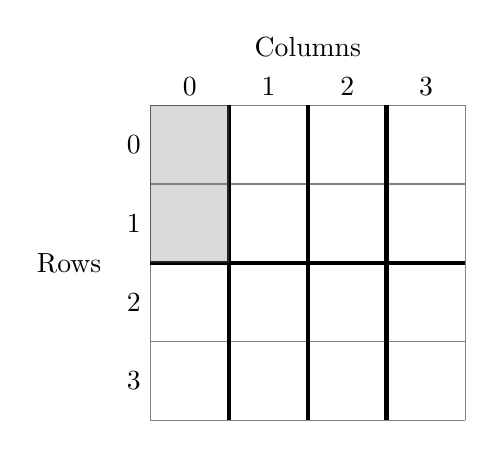
\begin{tikzpicture}

    \draw[step=1cm,gray] (0, 0) grid (4, 4);

    % Make the row numbers
    \foreach \x in {0,...,3}{
        \pgfmathsetmacro\y{int(3 - \x)};
        \node[left] at (0, \x + 0.5) {\y};
    }

    % Make the column numbers
    \foreach \x in {0,...,3}{
        \node[above] at (\x + 0.5, 4) {\x};
    }


    \node[left=0.5cm] at (0, 2) {Rows};
    \node[above=0.5cm] at (2, 4) {Columns};

    % Split rows
    \draw[ultra thick] (0, 2)--(4, 2);

    % Split columns
    \draw[ultra thick] (1, 0)--(1, 4);
    \draw[ultra thick] (2, 0)--(2, 4);
    \draw[ultra thick] (3, 0)--(3, 4);

    \draw[fill=gray, opacity=0.3] (0, 2) rectangle (1, 4);

    % \draw[fill=gray, opacity=.1] (0, 0) rectangle (2, 2);
    % \draw[fill=gray, opacity=.3] (0, 2) rectangle (2, 4);
    % \draw[fill=gray, opacity=.6] (2, 2) rectangle (4, 4);

\end{tikzpicture}
\end{document}